% !TEX root = ../../../Lazcorreta.Tesis.tex
% \ABIERTO%
\begin{wrapfigure}{o}{0.35\textwidth}
  \centering
  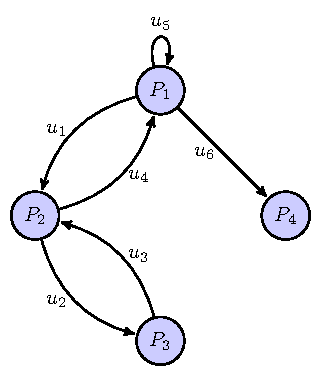
\includegraphics[width=.35\textwidth]{_MNW.pdf}
	\caption{\Sn}
	\label{fig:1-3-1-SN}
\end{wrapfigure}
Para analizar mejor una \sn vamos a dibujarla. Primero dibujamos un círculo representando $p_1$, luego dibujamos $p_2$ (si es distinta a $p_1$) y una flecha que va de $p_1$ a $p_2$ y en ella anotamos $u_1$. Seguimos dibujando las páginas que no estén ya en el dibujo y la flecha que la une con la anterior página dibujada, con su $u_i$ correspondiente. Cuando completamos el dibujo observamos que tenemos un \grafo compuesto y dirigido que modeliza una \sn y sobre el que se podrán aplicar muchos conocimentos derivados de la Teoría de Grafos.

Es un enfoque matemático para observar una \secuencia. Para crear cada \grafo hay que leer una \sn e ir agregando nodos y ejes a un \grafo vacío, considerando si ya existe el nodo a insertar. Los nodos son las páginas visitadas $p_j$, el tiempo $u_j$ que ha permanecido el usuario en dicha página es el peso del enlace a la siguiente página visitada en la sesión, $p_{j+1}$. La última página de la sesión no genera ningún eje. Cada sesión $s_i$, $i = 1 \ldots N$, se convierte en el \grafo $G_i$.

\begin{equation}\label{eq:1-3-1-grafoSesion}
   \begin{array}{ll}
      G_i = & \left( P', E' \right) \ | \\
            & P' = \left\{ P'_j, j = 1\ldots n_i \right\} \ \wedge \\
            & E' = \left\{ \left( E'_{jk}, u_j \right), 1 \leq j \leq n_{i-1}, 1 \leq k \leq n_i \right\} 
   \end{array}
\end{equation}

La representación gráfica de una \sn puede ayudar al analista a comprender mejor el uso que se hace del sitio web. Cada nodo hoja puede catalogarse como un \emph{objetivo} del usuario o un intento fallido tras el que decide volver por donde vino. Si permanece mucho tiempo en ese nodo es más probable que sea su objetivo, en cuyo caso deberíamos facilitarle acceso directo desde la página en que inició la búsqueda de su objetivo. Todos los nodos en que permanece mucho tiempo un usuario podrían catalogarse como objetivos en la sesión. Aquellos en que permanece poco tiempo se pueden catalogar como recursos intermedios que podrían no ser visitados si existieran enlaces directos a sus objetivos. Pero todo esto lo han de mostrar los propios datos, y en la fase de evaluación debería comprobarse la calidad de las estimaciones hechas.



% \begin{figure}
%    \centering
   % \begin{subfigure}[b]{0.3\textwidth}
   %    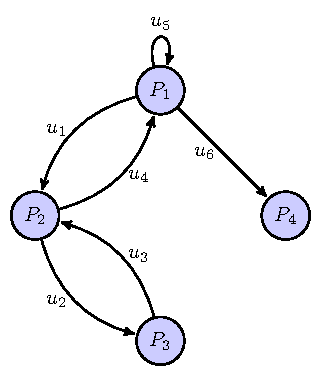
\includegraphics[width=\textwidth]{_MNW.pdf}
   %    \caption{\Sn}
   %    \label{fig:1-3-1-SN}
   % \end{subfigure}%
   % \hfill
   % \begin{subfigure}[b]{0.4\textwidth}
   %    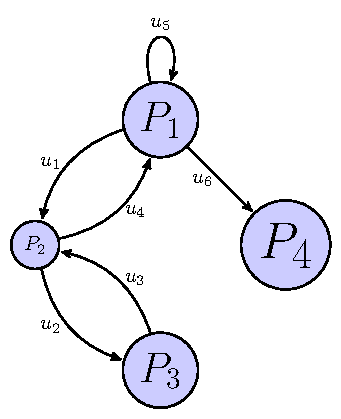
\includegraphics[width=\textwidth]{_MNWponderado.pdf}
   %    \caption{\ldots ponderada}
   %    \label{fig:1-3-1-SNPonderada}
   % \end{subfigure}
   % \hfill
%    \begin{subfigure}[b]{0.4\textwidth}
%       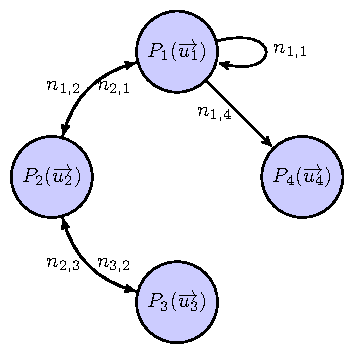
\includegraphics[width=\textwidth]{_MNW_articulo.pdf}
%       \caption{\MNW}
%       \label{fig:1-3-1-MNW}
%    \end{subfigure}
%    \caption{Construcción del \mnw}
%    \label{fig:1-3-1-SN2MNW}
% \end{figure}




\begin{wrapfigure}{o}{0.35\textwidth}
  \centering
  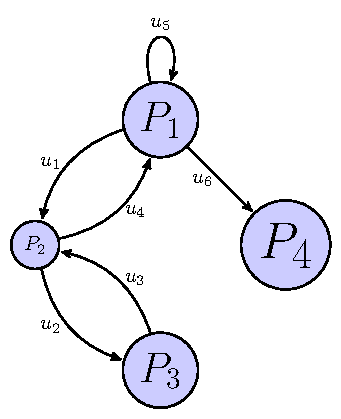
\includegraphics[width=.35\textwidth]{_MNWponderado.pdf}
	\caption{\Sn ponderada}
	\label{fig:1-3-1-SNPonderada}
\end{wrapfigure}
Si catalogamos cada página $P'_j$ como \emph{objetivo} o \emph{de transición} en función de su vector $\overrightarrow{u}_j$, definido mediante la ecuación~\ref{eq:1-2-4-tiempoPermanencia}, ya estamos haciendo estimaciones, intentando que sea un dato concreto, el tiempo de permanencia en una página, quien nos permita hacer una primera \clasificacion de las páginas del sitio web. Gráficamente se aprecia en seguida el efecto de esta \clasificacion, como muestra la figura~\ref{fig:1-3-1-SNPonderada}. Hemos de recordar que estamos trabajando con \DM por que serán muchos los \grafos que obtengamos, y además los queremos tratar en tiempo real por lo que este tipo de representaciones sólo se hará para que el analista pueda ver la información que tiene desde distintas perspectivas.
%TODO: Esta \clasificacion se fundamentaría en la hipótesis de que una página con tiempos bajos de permanencia parece ser que no ofrece su contenido al usuario (a no ser que sea un contenido muy breve, claro) si no que le ofrece la posibilidad de pasar a otra página en la que quizá esté lo que busca el usuario. En las páginas en que se detiene mucho tiempo el usuario se supone que es porque su contenido le resulta interesante. Se pueden plantear muchas hipótesis, lo que hay que lograr es un método que ayude al investigador a decidir si la hipótesis es confirmada por los datos disponibles. Para ayudarnos de forma visual podríamos ponderar el tamaño de los nodos del \grafo en función de si estimamos que son \emph{objetivo} o \emph{de transición}, como se muestra en la figura~\ref{fig:grafoMUW}.


No es casualidad que la estructura elegida sea un \grafo compuesto, es el efecto de utilizar papel y lápiz para dibujar una \sn. Sin embargo un \grafo compuesto utiliza muchos recursos de memoria para guardar los múltiples ejes que pueden unir dos nodos. Podemos guardar casi la misma información en un \grafo simple y dirigido cuyos nodos contienen la página visitada y el vector de tiempos de permanencia y sus ejes están ponderados con el número de veces que se ha usado ese enlace en esa sesión, como muestra la figura~\ref{fig:1-3-1-MNW}. En este caso no podremos relacionar los tiempos de permanencia con la página de la que proviene, al trabajar con \grafos compuestos sí teníamos esa información pero no sabíamos como usarla por lo que vamos a prescindir de ella trabajando con \grafos simples.

Incluso la información sobre $\overrightarrow{u}_j$ se podría sustituir por un único valor representativo del vector de tiempos de permanencia en la página $p_j$ (su media aritmética, moda\ldots). Depende del uso que le vayamos a dar puede ser conveniente sustituir todos esos datos por uno que los describa adecuadamente y liberar memoria para los costosos procesos de \dm a que vamos a someter los datos. Como en todo proceso de \KDD el valor utilizado para representar $\overrightarrow{u}_j$ puede producir variaciones sensibles en los resultados obtenidos por lo que se deberían hacer pruebas con diferentes valores representativos de esta variable hasta encontrar uno que proporcione conocimiento de mayor calidad.

Con todas estas transformaciones hemos definido el \mnw (\MNW), mostrado en la figura~\ref{fig:1-3-1-MNW}, del que queremos extraer toda la información posible sobre el uso del sitio web en estudio.

\begin{defn}[\emph{Mapa de Navegación Web}]\label{def:1-3-1-MNW}
  \begin{equation}\label{eq:1-3-1-MNW}
     \begin{array}{ll}
        MNW_i = & \left( P', E' \right) \ | \\
              & P' = \left\{ \left(P'_j, \overrightarrow{u}_j \right),\ j = 1\ldots n_i \right\} \ \wedge \\
              & E' = \left\{ \left( E'_{jk}, n_{jk} \right), 1 \leq j \leq n_{i-1}, 1 \leq k \leq n_i \right\} 
     \end{array}
  \end{equation}
\end{defn}


\begin{wrapfigure}{o}{0.35\textwidth}
  \centering
  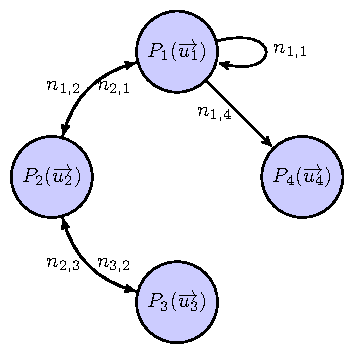
\includegraphics[width=.35\textwidth]{_MNW_articulo.pdf}
	\caption{\MNW}
\label{fig:1-3-1-MNW}
\end{wrapfigure}
Si tenemos el mapa del sitio web podemos comprobar qué enlaces existentes en $E$ no se utilizan y preguntarnos por qué. En muchas ocasiones es sólo por cuestión de su ubicación, tamaño o etiqueta (por no ser muy explícita o no estar bien redactada). Hay que recordar que si estamos trabajando en un sitio web que hace recomendaciones de forma dinámica los enlaces de $E$ cambiarán constantemente y estas comprobaciones podrían carecer de sentido si se analizan datos antiguos.

La unión de todos los \mnws de un mismo usuario proporciona su \mpnw, mostrado en la figura~\ref{fig:1-3-1-MPNW}.

\begin{defn}[\emph{Mapa Personal de Navegación Web}]\label{def:1-3-1-MPNW}
  \begin{equation}
     \label{eq:1-MPNW}
     MPNW_{userID} = \bigcup_{i=1}^{N}{MNW_i}\ | \ {sesion}_i.user = userID 
  \end{equation}
\end{defn}


En el \emph{Mapa Personal de Navegación Web} está recogida toda la información sobre las \sns realizadas por el usuario por lo que cada vez que el usuario solicita una página del sitio web se busca dicha página en su ${MPNW}_{userID}$ y, si está, se recomendarán algunas de las páginas que estén conectadas con la solicitada mediante un eje o un camino, de dos ejes como máximo para no ralentizar esta fase, ordenando las recomendaciones en función del tiempo de permanencia que tiene cada una de las páginas sugeridas en su ${MPNW}_{userID}$. Podemos ir más allá y extender la búsqueda de páginas a recomendar a otro nivel utilizando caminos más largos y comprobando si las nuevas sugerencias son mejor acogidas por los usuarios del sitio web.

\begin{figure}[htbp]
  \centering
  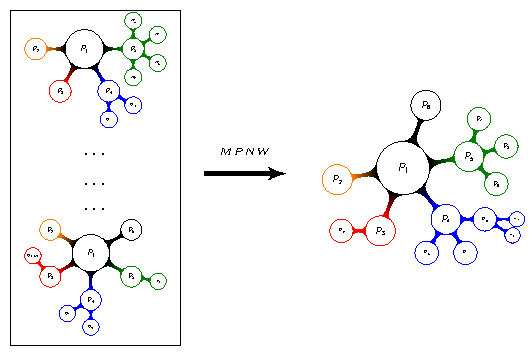
\includegraphics[width=.80\textwidth]{MPNW}
  \caption{Obtención del \MPNW}
\label{fig:1-3-1-MPNW}
\end{figure}





Si tenemos $m$ usuarios, $userID = 1\ldots m$, podemos modelizar el uso general del sitio web mediante la unión de todos sus $MPNW$, obteniendo un \musw (\MUSW).

\begin{defn}[\emph{Mapa de Uso del Sitio Web}]\label{def:1-3-1-MUSW}
  \begin{equation}\label{eq:1-3-1-MUSW}
    MUSW = \bigcup_{userID=1}^{m}{MPNW_{userID}} 
  \end{equation}
\end{defn}

El \MUSW se puede utilizar para hacer recomendaciones a usuarios que no hayan estado antes en nuestro sitio web, ya que no tendremos información sobre su \MPNW$_{userID}$. Se usará del mismo modo que usamos los mapas personales, buscando en el \grafo la página solicitada por el usuario y añadiéndole enlaces con recomendaciones basadas en los ejes que salen de dicha página en el \grafo, ponderadas por el tiempo de permanencia de las páginas destino de cada eje.

Si un usuario ya ha estado en nuestro sitio web con anterioridad y tenemos su \MPNW$_{userID}$ podemos ofrecerle mejor información si tenemos en cuenta tanto su \MPNW como el \MUSW. Para hacerlo en tiempo real nos hemos de limitar a consultar únicamente qué enlaces tiene la página solicitada por el usuario en ambos mapas y extraer inmediatamente el mejor conocimiento de estos datos. 

Estamos intentando trabajar con muchos datos simultáneamente. Al catalogar las páginas se consigue una gran reducción de datos, si no se pierde información habremos hecho un gran avance. Aún así seguimos trabajando con muchos datos, sería deseable poder dividir el gran conjunto de \grafos que queremos analizar en conjuntos más pequeños y gestionables. Existen para ello muchas técnicas de \clustering~\citep{NgHan-EfficientAndEffectiveClusteringMethods-1994}, la idea siempre es la misma: agrupar a los individuos que más se parezcan entre sí y más se diferencien del individuo representativo de los otros grupos. La cuestión es ahora determinar qué función de "`similitud"' se debe aplicar a nuestros mapas de navegación y cuál será su coste computacional.

Nuestros \grafos están compuestos por las páginas del sitio web, los enlaces utilizados para navegar a través de ellas y el tiempo estimado de permanencia en cada página (o su catalogación como \emph{objetivo} o \emph{de transición} o \emph{intento fallido}). ¿Cómo determinamos que dos \sns son "`parecidas"'? En primer lugar deberíamos observar si contienen los mismos nodos, si se han visitado las mismas páginas o al menos un conjunto de ellas coinciden, a continuación podríamos observar la similitud en cuanto a tiempo de permanencia en las páginas visitadas en ambas sesiones y, por último, la coincidencia en el uso de enlaces haría más próximos ambos \grafos. Comparar todos estos datos en una colección grande de \grafos no es tarea trivial, no podemos esperar resultados en tiempo real pues hay que hacer muchas operaciones complejas para determinar si dos \grafos son similares:
\begin{enumerate}
   \item calcular su intersección, comprobar qué páginas del primer \grafo están en el segundo,
   \item comprobar si la intersección obtenida es representativa para ambos \grafos,
   \item comparar los tiempos de permanencia en las páginas seleccionadas,
   \item comprobar si los enlaces utilizados en ambas sesiones presentan similitudes.
\end{enumerate}

Si trasladamos esto a la comparación de más de dos \grafos se complica el asunto. La intersección de muchos \grafos puede no contener ningún nodo con lo que habríamos perdido toda la información disponible. Al obtener la intersección de dos \grafos deberíamos considerar también los nodos (páginas visitadas) que no pertenecen a la intersección pero sí a uno de los \grafos, lo que se podría conseguir a nivel de usuario haciendo la intersección de un \grafo con el \mpnw del usuario o con el \musw y considerando los nodos adyacentes a estas intersecciones en el mapa utilizado como posibles páginas a recomendar al usuario.

A pesar de disponer de muchas herramientas de Teoría de Grafos para llevar a cabo el estudio actual, al poner a prueba nuestra propuesta no se pudieron guardar todos los resultados obtenidos para poder manipularlos en tiempo real. Uno de los retos de la \dm es extraer de enormes cantidades de datos la máxima información siendo conscientes de que trabajamos siempre con recursos limitados, lo que nos hizo replantear el análisis propuesto reduciendo de nuevo los datos a gestionar. Aunque los enlaces utilizados por los usuarios son quienes nos dan más información sobre la navegación a través de nuestro sitio web decidimos prescindir de ellos para centrarnos en analizar las páginas visitadas en una \sn, sin conservar el orden en que se visitó cada página ni el tiempo de permanencia estimado para cada una de ellas. Aún así el número de datos a gestionar era muy grande por lo que tuvimos que buscar metodologías aplicables a esta nueva situación.

